% Options for packages loaded elsewhere
\PassOptionsToPackage{unicode}{hyperref}
\PassOptionsToPackage{hyphens}{url}
\PassOptionsToPackage{dvipsnames,svgnames,x11names}{xcolor}
%
\documentclass[
  a4paper,
]{article}

\usepackage{amsmath,amssymb}
\usepackage{setspace}
\usepackage{iftex}
\ifPDFTeX
  \usepackage[T1]{fontenc}
  \usepackage[utf8]{inputenc}
  \usepackage{textcomp} % provide euro and other symbols
\else % if luatex or xetex
  \usepackage{unicode-math}
  \defaultfontfeatures{Scale=MatchLowercase}
  \defaultfontfeatures[\rmfamily]{Ligatures=TeX,Scale=1}
\fi
\usepackage[]{times}
\ifPDFTeX\else  
    % xetex/luatex font selection
\fi
% Use upquote if available, for straight quotes in verbatim environments
\IfFileExists{upquote.sty}{\usepackage{upquote}}{}
\IfFileExists{microtype.sty}{% use microtype if available
  \usepackage[]{microtype}
  \UseMicrotypeSet[protrusion]{basicmath} % disable protrusion for tt fonts
}{}
\makeatletter
\@ifundefined{KOMAClassName}{% if non-KOMA class
  \IfFileExists{parskip.sty}{%
    \usepackage{parskip}
  }{% else
    \setlength{\parindent}{0pt}
    \setlength{\parskip}{6pt plus 2pt minus 1pt}}
}{% if KOMA class
  \KOMAoptions{parskip=half}}
\makeatother
\usepackage{xcolor}
\usepackage[margin=1in]{geometry}
\setlength{\emergencystretch}{3em} % prevent overfull lines
\setcounter{secnumdepth}{5}
% Make \paragraph and \subparagraph free-standing
\ifx\paragraph\undefined\else
  \let\oldparagraph\paragraph
  \renewcommand{\paragraph}[1]{\oldparagraph{#1}\mbox{}}
\fi
\ifx\subparagraph\undefined\else
  \let\oldsubparagraph\subparagraph
  \renewcommand{\subparagraph}[1]{\oldsubparagraph{#1}\mbox{}}
\fi


\providecommand{\tightlist}{%
  \setlength{\itemsep}{0pt}\setlength{\parskip}{0pt}}\usepackage{longtable,booktabs,array}
\usepackage{calc} % for calculating minipage widths
% Correct order of tables after \paragraph or \subparagraph
\usepackage{etoolbox}
\makeatletter
\patchcmd\longtable{\par}{\if@noskipsec\mbox{}\fi\par}{}{}
\makeatother
% Allow footnotes in longtable head/foot
\IfFileExists{footnotehyper.sty}{\usepackage{footnotehyper}}{\usepackage{footnote}}
\makesavenoteenv{longtable}
\usepackage{graphicx}
\makeatletter
\def\maxwidth{\ifdim\Gin@nat@width>\linewidth\linewidth\else\Gin@nat@width\fi}
\def\maxheight{\ifdim\Gin@nat@height>\textheight\textheight\else\Gin@nat@height\fi}
\makeatother
% Scale images if necessary, so that they will not overflow the page
% margins by default, and it is still possible to overwrite the defaults
% using explicit options in \includegraphics[width, height, ...]{}
\setkeys{Gin}{width=\maxwidth,height=\maxheight,keepaspectratio}
% Set default figure placement to htbp
\makeatletter
\def\fps@figure{htbp}
\makeatother
\newlength{\cslhangindent}
\setlength{\cslhangindent}{1.5em}
\newlength{\csllabelwidth}
\setlength{\csllabelwidth}{3em}
\newlength{\cslentryspacingunit} % times entry-spacing
\setlength{\cslentryspacingunit}{\parskip}
\newenvironment{CSLReferences}[2] % #1 hanging-ident, #2 entry spacing
 {% don't indent paragraphs
  \setlength{\parindent}{0pt}
  % turn on hanging indent if param 1 is 1
  \ifodd #1
  \let\oldpar\par
  \def\par{\hangindent=\cslhangindent\oldpar}
  \fi
  % set entry spacing
  \setlength{\parskip}{#2\cslentryspacingunit}
 }%
 {}
\usepackage{calc}
\newcommand{\CSLBlock}[1]{#1\hfill\break}
\newcommand{\CSLLeftMargin}[1]{\parbox[t]{\csllabelwidth}{#1}}
\newcommand{\CSLRightInline}[1]{\parbox[t]{\linewidth - \csllabelwidth}{#1}\break}
\newcommand{\CSLIndent}[1]{\hspace{\cslhangindent}#1}

\usepackage[noblocks]{authblk}
\usepackage{subcaption}
\usepackage{lineno}
\renewcommand*{\Authsep}{, }
\renewcommand*{\Authand}{, }
\renewcommand*{\Authands}{, }
\renewcommand\Affilfont{\small}
\usepackage{lscape}
\newcommand{\blandscape}{\begin{landscape}}
\newcommand{\elandscape}{\end{landscape}}
\makeatletter
\makeatother
\makeatletter
\makeatother
\makeatletter
\@ifpackageloaded{caption}{}{\usepackage{caption}}
\AtBeginDocument{%
\ifdefined\contentsname
  \renewcommand*\contentsname{Table of contents}
\else
  \newcommand\contentsname{Table of contents}
\fi
\ifdefined\listfigurename
  \renewcommand*\listfigurename{List of Figures}
\else
  \newcommand\listfigurename{List of Figures}
\fi
\ifdefined\listtablename
  \renewcommand*\listtablename{List of Tables}
\else
  \newcommand\listtablename{List of Tables}
\fi
\ifdefined\figurename
  \renewcommand*\figurename{Figure}
\else
  \newcommand\figurename{Figure}
\fi
\ifdefined\tablename
  \renewcommand*\tablename{Table}
\else
  \newcommand\tablename{Table}
\fi
}
\@ifpackageloaded{float}{}{\usepackage{float}}
\floatstyle{ruled}
\@ifundefined{c@chapter}{\newfloat{codelisting}{h}{lop}}{\newfloat{codelisting}{h}{lop}[chapter]}
\floatname{codelisting}{Listing}
\newcommand*\listoflistings{\listof{codelisting}{List of Listings}}
\makeatother
\makeatletter
\@ifpackageloaded{caption}{}{\usepackage{caption}}
\@ifpackageloaded{subcaption}{}{\usepackage{subcaption}}
\makeatother
\makeatletter
\@ifpackageloaded{tcolorbox}{}{\usepackage[skins,breakable]{tcolorbox}}
\makeatother
\makeatletter
\@ifundefined{shadecolor}{\definecolor{shadecolor}{rgb}{.97, .97, .97}}
\makeatother
\makeatletter
\makeatother
\makeatletter
\makeatother
\ifLuaTeX
  \usepackage{selnolig}  % disable illegal ligatures
\fi
\IfFileExists{bookmark.sty}{\usepackage{bookmark}}{\usepackage{hyperref}}
\IfFileExists{xurl.sty}{\usepackage{xurl}}{} % add URL line breaks if available
\urlstyle{same} % disable monospaced font for URLs
\hypersetup{
  pdftitle={Microbial network inference},
  pdfauthor={Francisco Campuzano Jiménez},
  colorlinks=true,
  linkcolor={blue},
  filecolor={Maroon},
  citecolor={Blue},
  urlcolor={Blue},
  pdfcreator={LaTeX via pandoc}}

\title{Microbial network inference}


  \author{Francisco Campuzano Jiménez}
            \affil{%
                  Bioinformatics Research Centre, Aarhus University
              }
      
\date{2023-12-28}
\begin{document}
\maketitle
\ifdefined\Shaded\renewenvironment{Shaded}{\begin{tcolorbox}[boxrule=0pt, frame hidden, sharp corners, enhanced, breakable, interior hidden, borderline west={3pt}{0pt}{shadecolor}]}{\end{tcolorbox}}\fi

\setstretch{1.25}
\newpage
\linenumbers

\hypertarget{introduction}{%
\section{Introduction}\label{introduction}}

The recent advances in microbial amplicon and metagenomic sequencing
produce extensive collections of co-occurrence data suitable for
quantitative analysis (Badri et al. 2020). Microbial taxa associations
\emph{in situ} can not usually be assessed by observing interactions as
in macro-ecosystems (Guseva et al. 2022). Therefore, methods based on
co-occurrence data and their interpretation are an active and
controversial research topic (Blanchet, Cazelles, and Gravel 2020).

Microbial networks are temporary or spatial snapshots of ecosystems,
where we display taxonomic units as nodes (but also environmental
variables) and significant associations as undirected edges (Röttjers
and Faust 2018). Many inference methods in the literature are based on
pairwise correlation-based or graphical models (Matchado et al. 2021).
This work focuses on the latter, as they are less affected by correlated
but indirectly connected taxa\footnote{Let us consider three random
  variables, A, B, and C, that correspond to the abundances of three
  OTUs. Assume that \(\Pr(A |BC) = \Pr(A |B)\), \(\Pr(B |AC) = \Pr(B)\)
  and \(\Pr(C |AB) = \Pr(C |B)\). The edge \((A, C)\) is what the
  literature commonly defines as indirectly connected nodes (through
  \(B\) in this example.}.

The sequencing bioinformatics pipeline determines the exact meaning of
the nodes, as raw reads can be clustered into operational taxonomic
units, kept separated as amplicon sequence variants, and agglomerated
into higher taxonomic levels (Bharti and Grimm 2021). The biological
meaning of networks has been qualified as ``uncertain'' and requires
careful interpretation of all prior steps and their impact on the
outcome (Faust 2021).

Microbial inference algorithms are known to return so-called hairballs
(intricate and densely interconnected graphs) (Faust 2021; Röttjers and
Faust 2018). Some authors claimed it is necessary to estimate and
analyze the network properties to gain biological insights from
co-occurrence networks (Röttjers and Faust 2018; Abu-Mostafa,
Magdon-Ismail, and Lin 2012).

For example, at the network level, we can study whether some species
tend to co-occur with each other more often, quantified by the
modularity\footnote{Formally,
  \(Q = \frac{1}{2m}\sum_{ij}\left( A_{ij} - \gamma \frac{k_ik_j}{2m}\right )\mathbb1_{c_i = c_j}\),
  where \(m\) is the number of edges, \(A\) is the adjacency matrix,
  \(k_x\) is the degree of the \(x\) node and \(c_x\) the cluster of the
  \(x\) node (Clauset, Newman, and Moore 2004).} or how well the
degree\footnote{The degree of a node is simply the number of edges it
  has (Hansen, Shneiderman, and Smith 2011).} distribution fits a null
distribution (Guseva et al. 2022). At the node level, on the other hand,
we can analyze the relation between network distances\footnote{The
  shortest between two nodes is the path with the minimal number of
  edges.} and phylogenetic similarity (Morueta-Holme et al. 2016), as
well as node centrality. However, it is unreasonable to assume that
highly connected nodes in the network show any evidence of those taxa
being keystone\footnote{``A species whose impact on its community or
  ecosystem is large, and disproportionately large relative to its
  abundance'' (Power et al. 1996).} species (Röttjers and Faust 2018;
Guseva et al. 2022). Therefore, we advise not using centrality
measurements such as the hub score\footnote{The hub scores are defined
  for undirected networks as the principal eigenvector of \(A^\top A\),
  where \(A\) is the adjacency matrix Kleinberg (1998a).} to identify
keystone taxa, even though they are frequently used. Instead, centrality
measurements should be used as an indicator of whether certain OTUs have
broader niche preferences than others.

The use of undirected Gaussian graphical models in this field has become
increasingly popular. This work focuses on studying how reliable the
results derived from network inference under typical conditions of
working with environmental samples characterized by a limited number of
samples. We have compared two methods, SpiecEASI (Kurtz et al. 2015),
the most popular approach, and one novel Bayesian alternative based on
the BDgraph package (R. Mohammadi and Wit 2019).

\hypertarget{background}{%
\section{Background}\label{background}}

\begin{figure}

\begin{minipage}[t]{0.50\linewidth}

{\centering 

\raisebox{-\height}{

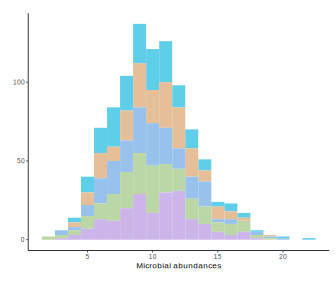
\includegraphics{report_files/mediabag/../figures/00-conceptual_figures/abundances.pdf}

}

}

\subcaption{\label{fig-conceptual-1}}
\end{minipage}%
%
\begin{minipage}[t]{0.50\linewidth}

{\centering 

\raisebox{-\height}{

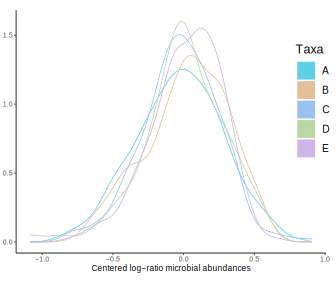
\includegraphics{report_files/mediabag/../figures/00-conceptual_figures/clr.pdf}

}

}

\subcaption{\label{fig-conceptual-2}}
\end{minipage}%
\newline
\begin{minipage}[t]{0.50\linewidth}

{\centering 

\raisebox{-\height}{


\includegraphics{report_files/mediabag/../figures/00-conceptual_figures/precision_mat.pdf}

}

}

\subcaption{\label{fig-conceptual-3}}
\end{minipage}%
%
\begin{minipage}[t]{0.50\linewidth}

{\centering 

\raisebox{-\height}{

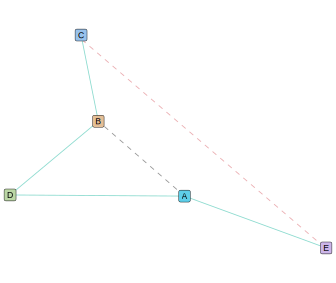
\includegraphics{report_files/mediabag/../figures/00-conceptual_figures/graph.pdf}

}

}

\subcaption{\label{fig-conceptual-4}}
\end{minipage}%

\caption{\label{fig-conceptual}\textbf{Inferring a microbial network
involves transforming the data and determining the graph structure from
a sparse precision matrix estimate.} (a) Abundances of five different
taxa across 200 samples, simulated according to a negative binomial
process with unequal depth between samples. (b) Centered log-ratio
abundances to address compositionality and the assumption of normality.
(c) Graphical lasso estimation of the precision matrix
(\(\lambda = 0.26\)). (d) Graph structure that corresponds to the
zero-pattern of \(\hat \Omega(\lambda = 0.26)\). False positive edges
are shown in light red, and false negatives in gray.}

\end{figure}

\hypertarget{gaussian-graphical-models}{%
\subsection{Gaussian graphical models}\label{gaussian-graphical-models}}

We adapted the definition of Gaussian graphical models from Uhler
(2017). Let \(G = (V, E)\) be an undirected graph with nodes
\(V=\{1, \dots, p\}\) and edges
\(E \subset \{(i, j) \in V\times V : i<j\}\). In our application
context, \(V\) is the set of microbial taxa. We define the edges of the
graph such that the absence of edge \((i, j)\) implies conditional
independence between the taxon \(i\) and \(j\) given all the other
variables.

It is possible to infer the graph by first estimating the inverse of the
covariance matrix, known as the precision matrix,
\(\Omega:= \Sigma^{-1}\). The precision matrix is useful because, for
every matrix element, it is true that \(\Omega_{ij}=0\) if and only if
the \(i\) and \(j\) are conditionally independent given the rest of the
dimensions. Then, we can unambiguously determine the graph structure
from the pattern of zero entries in the precision matrix
(Figure~\ref{fig-conceptual-3} and Figure~\ref{fig-conceptual-4}).
Formally, we say that a random variable \(X \in \mathbb R_p\) follows
\(G = (V, E)\) if it is distributed as
\(\mathcal N_p(0, \Omega ^{-1})\), where \(\Omega\) is a positive
definite matrix of dimensions \(p\times p\) such that
\(\Omega_{ij} = 0\) implies \((i, j) \notin E\).

Research inferring microbial networks using graphical models has focused
exclusively on estimating sparse Gaussian graphical models. The most
popular idea is to induce sparsity by imposing a \(L_1\) penalty on the
precision matrix. This approach has succeeded in the likelihood
framework under the name of graphical lasso (Friedman, Hastie, and
Tibshirani 2008).

\hypertarget{data-transformation}{%
\subsection{Data transformation}\label{data-transformation}}

Unfortunately, microbial abundance data is not normal
(Figure~\ref{fig-conceptual-1}). In the literature, methods overcome
this issue by applying some transformation over the original discrete
counts. Alternatively, methods that simultaneously estimate the
precision matrix and a set of \(p\) normal latent variables from the
\(p\) observed variables are known as Copula Gaussian graphical models.

Even worse, microbial abundance data is highly compositional because of
unequal depth and sampling. To compare abundances between samples, the
observed counts, \(\hat W\in \mathbb N_{n \times p}\), are often
normalized by the total sum of counts per sample
Equation~\ref{eq-relative}.

\begin{equation}\protect\hypertarget{eq-relative}{}{
X_{ij} = \frac{\hat W_{ij}}{\sum_{m=1}^n \hat W_{im}}
}\label{eq-relative}\end{equation}

However, this normalization imposes a sum-to-one constraint, making the
relative abundances, \(X \in \mathbb R^+_{n\times p}\), of the different
taxa no longer independent. Kurtz et al. (2015) proposed to apply the
centered log-ratio transformation (see Equation~\ref{eq-clr}) to the
relative abundances and estimate the Gaussian graphical model from the
transformed data \(X \in \mathbb R_{n\times p}\)
(Figure~\ref{fig-conceptual-4}). This transformation is by far the most
widely used.

\begin{equation}\protect\hypertarget{eq-clr}{}{
Z_{ij} = \log \left (\frac{X_{ij}}{\left [ \prod_{m=1}^pX_{im}\right]^{\frac 1 p}}\right )
}\label{eq-clr}\end{equation}

Let us denote the per-sample total counts sum as
\(m_i = \sum_{m=1}^p W_{i,m}\). The intuition behind the centered
log-ratio transformation is that because
\(\log{\frac {W_{i*}}{W_{j*}}} = \log{\frac {W_{i*}/m_*}{W_{j*}/m_*}} = \log{\frac {X_{i*}}{X_{j*}}}\),
the statistical inference done with the log ratios of relative
abundances are equivalent to the one done with the log ratio of
unobserved absolute abundances.

SpiecEASI\footnote{SpiecEASI stands for \textbf{SP}arse
  \textbf{I}nvers\textbf{E C}ovariance \textbf{E}stimation for
  ecological \textbf{AS}sociation \textbf{I}nference}, the most popular
tool for inferring Gaussian graphical models from microbial abundance
data, uses the centered-log ratio approach (Kurtz et al. 2015). However,
this transformation is not exempt from criticism. Because of numerical
problems with the geometric mean of the samples in
Equation~\ref{eq-clr}, SpiecEASI uses pseudo-counts instead of the
original values. When data is zero-inflated, the transformed data will
exhibit a peak corresponding to the spike at zero, which violates the
normality assumption and might lead to spurious associations (Ha et al.
2020).

\hypertarget{inferring-sparse-graph}{%
\subsection{Inferring sparse graph}\label{inferring-sparse-graph}}

\hypertarget{likelihood-framework}{%
\subsubsection{Likelihood framework}\label{likelihood-framework}}

In the likelihood framework, inferring the sparse Gaussian graphical
model is usually formulated according to Friedman, Hastie, and
Tibshirani (2008):

\begin{equation}\protect\hypertarget{eq-glasso}{}{
\begin{aligned}
\mathcal L(\Omega) = \log |\Omega| - \text{trace}(\hat \Sigma \Omega)\\
\hat \Omega(\lambda) = \arg \min_{\Omega\in M^+} (-L(\Omega) + \lambda ||\Omega||_1)
\end{aligned}
}\label{eq-glasso}\end{equation}

where \(M^+\) is the set of positive definite matrices, \(\hat \Sigma\)
is the empirical covariance matrix, and \(||\Omega||_1\) is the \(L_1\)
norm (the sum of all absolute values of the matrix).
\(\mathcal L(\Omega)\) is the log-likelihood of the data after
maximizing over the mean vector \(\mu\) and ignoring constants.
\(\lambda\) is a positive regularization parameter that controls the
sparsity of the estimated precision matrix, \(\hat \Omega(\lambda)\),
and, consequently, of the graph \(G(\lambda)\).

Friedman, Hastie, and Tibshirani (2008) proposed an algorithm that
efficiently solves the optimization problem shown in
Equation~\ref{eq-glasso}, frequently referred to as graphical lasso (or
glasso). Before that, Meinshausen and Bühlmann (2006) had already
proposed a method for estimating networks from a regularized precision
matrix. Instead of estimating the whole matrix, they proposed estimating
the patterns of zero elements by fitting \(p\) lasso regressions and
using each variable as the response variable. Let us denote as
\(\hat\beta_a^b\) the \(a\)-coefficient of the lasso regression with the
\(b\) variable as the response for a given value of \(\lambda\). They
constrained the estimated graph by excluding all the edges \((i, j)\)
where either \(\hat\beta_i^j = 0\) or \(\hat\beta_j^i = 0\).

Almost always, the sparsity of the true graph, thus, of the true unknown
precision matrix, is unknown. The challenge that likelihood methods to
infer microbial Gaussian graphical models face is selecting an
appropriate value of \(\lambda\). Different criteria might be used, such
as selecting \(\lambda\) so it optimizes the Akaike information
criterion, the Bayesian information criterion, or the largest within one
standard error of the optimal negative likelihood when doing cross-fold
validation (or any equivalent rule of thumb). However, since the
publication of the SPIEC-EASI method (Kurtz et al. 2015), nearly all
research microbial co-occurrence network inferences have used the
StARS\footnote{StARS stands for Stability Approach to Regularization
  Selection.} selection method (Liu, Roeder, and Wasserman 2010).

The StARS method is a general procedure that could be applied to any
graph inference method. However, Liu, Roeder, and Wasserman (2010) built
it on top of the Meinshausen and Bühlmann method. Despite its
simplicity, it gives better results than solving the graphical lasso in
terms of speed, sensitivity, and accuracy.

The core idea of StARS is to draw many random overlapping subsamples
(without replacement) and apply the Meinshausen and Bühlmann method for
each subsample with decreasing values of \(\lambda\) until there is a
small but acceptable amount of variability. They defined the variability
in terms of the average total instability of the edges. Specifically,
for any chosen \(\lambda\), they estimate \(m\) graphs, one from each
\(m\) subsample. They calculate the instability of a particular edge
\((i, j)\) as the fraction of every possible pair of those \(m\) graphs
that disagree in the presence or absence of the \((i, j)\) edge (Liu,
Roeder, and Wasserman 2010).

Liu, Roeder, and Wasserman (2010) claimed they could estimate a graph
containing the true graph with high probability by selecting the largest
value of \(\lambda\) (the most sparse graph) for which the average total
instability equals or less than \(\beta\). They claimed that this
cut-point \(\beta\) is an interpretable quantity (so they did not just
replace the problem of choosing \(\lambda\) to choose \(\beta\)) and
that a reasonable default value is \(\beta = 0.05\).

\hypertarget{bayesian-framework}{%
\subsubsection{Bayesian framework}\label{bayesian-framework}}

Wang (2012) were the first to introduce a Bayesian version of the
graphical lasso estimator Equation~\ref{eq-glasso}. Although there are
many alternatives, the main idea is to encode every value into an
appropriate hierarchical model and use Markov Chain Monte Carlo (MCMC)
to estimate the posterior distributions (Richard Li, McCormick, and
Clark 2019; Li, Craig, and Bhadra 2019; Piironen and Vehtari 2017).
Bayesian methods do not need to select a value for \(\lambda\). Instead,
\(\lambda\) can be included in the model, with a prior that expresses
the researcher's beliefs about the sparsity of the graph, and all
inference is done by marginalizing across its value (Jongerling,
Epskamp, and Williams 2023).

Bayesian graphical lasso models are very attractive for estimating the
precision matrix. However, all suffer from the same problem: because
priors place no probability in any value being exactly zero,
\(\Omega_{ij}=0\), there is no probability of the event
\(\Omega_{ij}=0\) in the posterior either. When inferring microbial
networks, we aim to estimate the graph, not the precision matrix. These
methods require a \emph{post hoc} heuristic on including or excluding an
edge of the inferred sparse graph. For example, set all off-diagonal
elements to zero if the 95\% credibility interval contains the zero
value (Jongerling, Epskamp, and Williams 2023).

The alternative is to use a family of priors called G-Wishart, a
discrete and continuous mixture prior distribution. If so, we estimate
the joint posterior distribution of the precision matrix and the graph
(Equation~\ref{eq-join-post}).

\begin{equation}\protect\hypertarget{eq-join-post}{}{
P(G, \Omega|Z) \propto P(Z|G, \Omega) P(\Omega|G)P(G)
}\label{eq-join-post}\end{equation}

Many priors have been proposed for the graph structure (A. Mohammadi and
Wit 2015; Carvalho and Scott 2009; Jones et al. 2005). One popular
choice depends on a \(\theta \in (0, 1)\) parameter that expresses our
prior belief in the sparsity of the graph (see Equation~\ref{eq-probg}).
Notice that if \(\theta = 0.5\), the distribution corresponds to the
uniform distribution over the whole graph space.

\begin{equation}\protect\hypertarget{eq-probg}{}{
P(G) \propto \left ( \frac{\theta}{1-\theta}\right) ^{|E|}
}\label{eq-probg}\end{equation}

The G-Wishart distribution is a convenient prior choice for the
precision matrix because it is conjugated with the likelihood function
of a multivariate normal distribution (Roverato 2002). The G-Wishart
prior of a given graph, \(W_G(b, D)\), depends on the number of degrees
of freedom \(b>2\) and a matrix \(D\in M^+\) that is usually set to be
the identity matrix. Equation~\ref{eq-probomega} shows how to calculate
the probability of the precision matrix given a graph. Notice that we
ensure \(\Omega\) is a valid precision matrix by multiplying the
probability by the indicator variable \(\mathbb 1_{\Omega\in M ^+}\)
(i.e., set to zero the probability of any nonpositive definite matrix).

\begin{equation}\protect\hypertarget{eq-probomega}{}{
P(\Omega|G) \propto |\Omega|^{(b-2)/2} \exp\left \{ -\frac 1 2 \text{trace}(D\Omega)  \right\} \mathbb 1_{\Omega\in M ^+}
}\label{eq-probomega}\end{equation}

We need a particular type of algorithm, the so-called Trans-dimensional
MCMC, to explore the graph space and estimate the model parameters
simultaneously. The issue with this approach is that the graph space
grows exponentially\footnote{Concretely, there are \(2^{p(p-1)/2}\)
  graphs.} with the number of nodes/taxa, and convergence is complex. A.
Mohammadi and Wit (2015) proposed a birth-death MCMC that works well in
practice. Every edge is added or removed according to an independent
birth and death Poisson process. The main idea is that the algorithm is
formulated such that the posterior distribution of a graph is
proportional to how long the sampling algorithm stayed in a particular
graph. In opposition to the frequentist approach we presented in the
previous section, this method does not perform graph selection but graph
search.

\hypertarget{methods}{%
\section{Methods}\label{methods}}

All code is contained in
\href{https://github.com/currocam/microbial-network-inference}{github.com/currocam/microbial-network-inference}.

\hypertarget{simulation-of-synthetic-datasets}{%
\subsection{Simulation of synthetic
datasets}\label{simulation-of-synthetic-datasets}}

Random networks were simulated by assigning a Bernoulli random variable
where \(p\) was fixed for every network and it was drawn from a uniform
distribution between 0.01 and 0.1. Hub networks were simulated by
assigning each node to a random \(g\) group. Each group is then assigned
a center (from itself), and one edge is inserted for every node with its
center. The number of hubs, \(g\), was randomly chosen to be an integer
from one to ten. Cluster networks were simulated by assigning each node
to a random \(g\) group (again, sampled from 1 to 10). Then, we assigned
a Bernoulli random variable with \(p=0.2\) between every pair of nodes
that belongs to the same group.

We used BDgraph to simulate data from a negative binomial distribution
such that its correlations were consistent with the simulated graphs (R.
Mohammadi and Wit 2019). We simulated unequal depth sequencing by
multiplying with a correction factor (chosen uniformly between 0.75 and
1.25).

\hypertarget{fitting-graphical-models-with-spieceasi}{%
\subsection{Fitting graphical models with
SpiecEASI}\label{fitting-graphical-models-with-spieceasi}}

We fitted graphical models using the Pulsar implementation (Müller,
Bonneau, and Kurtz, n.d.), as described by Kurtz et al. (2015) (although
a Julia implementation was also made).

\hypertarget{fitting-graphical-models-with-bdgraph}{%
\subsection{Fitting graphical models with
BDgraph}\label{fitting-graphical-models-with-bdgraph}}

We used the birth-death MCMC algorithm (R. Mohammadi and Wit 2019), with
10000 iterations (and 5000 burn-in iterations). We assign an
uninformative prior to the graph space (all graphs are equally
plausible) but the initial graph is empty. The chosen G-Wishart prior
distribution has two degrees. We assessed the convergence by tracing the
number of edges across the chain. Results were robust between
hyperparameters.

\hypertarget{network-properties}{%
\subsection{Network properties}\label{network-properties}}

All network properties were computed using the igraph implementation
(Csardi and Nepusz 2006). The computed modularities according to the
community structure we found using short random walks (Pons and Latapy,
n.d.). We computed Kleinberg's hub score and scaled it so one is the
maximum score (Kleinberg 1998b). When computing similarity between
clusters partition, we first found the clusters using short random walks
(Pons and Latapy, n.d.) and then computed the adjusted mutual
information as implemented in the aricode R package (Vinh, Epps, and
Bailey 2009).

\hypertarget{results}{%
\section{Results}\label{results}}

\hypertarget{simulation-of-synthetic-datasets-1}{%
\subsection{Simulation of synthetic
datasets}\label{simulation-of-synthetic-datasets-1}}

As the popularity of microbial co-occurrence networks has increased,
more and more methods have been published in the last few years. Despite
this, there is no accepted experimental or simulated dataset to
reference when comparing the performance of different methods (Matchado
et al. 2021). We simulated data for different graph sizes and three
network topologies (see Figure~\ref{fig-networks}). First, we simulated
normal multivariate data such that their precision matrix was compatible
with the graph (the opposite of what we do during inference). Then, we
simulated correlated microbial abundances from the normal multivariate
distribution. The abundance of every taxon was drawn from a negative
binomial distribution and unequal depth between samples.

\begin{figure}

\begin{minipage}[t]{0.50\linewidth}

{\centering 

\raisebox{-\height}{

\includegraphics{../figures/11-network_plots/random_500.pdf}

}

}

\subcaption{\label{fig-random1}Random network (Graph size = 193)}
\end{minipage}%
%
\begin{minipage}[t]{0.50\linewidth}

{\centering 

\raisebox{-\height}{

\includegraphics{../figures/11-network_plots/random_100.pdf}

}

}

\subcaption{\label{fig-random2}Random network (Graph size = 120)}
\end{minipage}%
\newline
\begin{minipage}[t]{0.50\linewidth}

{\centering 

\raisebox{-\height}{

\includegraphics{../figures/11-network_plots/cluster_100.pdf}

}

}

\subcaption{\label{fig-cluster}Cluster network (Graph size = 184)}
\end{minipage}%
%
\begin{minipage}[t]{0.50\linewidth}

{\centering 

\raisebox{-\height}{

\includegraphics{../figures/11-network_plots/hub_100.pdf}

}

}

\subcaption{\label{fig-hub}Hub network (Graph size = 294)}
\end{minipage}%

\caption{\label{fig-networks}We analyzed three representative network
topologies: random, hub, and cluster. Subfigures show four randomly
simulated networks with 100 nodes (taxonomic units) and a different
number of edges (graph size). More details on its simulation in
methods.}

\end{figure}

\hypertarget{recovery-of-microbial-networks}{%
\subsection{Recovery of microbial
networks}\label{recovery-of-microbial-networks}}

\begin{figure}

\begin{minipage}[t]{\linewidth}

{\centering 

\raisebox{-\height}{

\includegraphics{../figures/01-precision-recall/f1-normal.pdf}

}

}

\subcaption{\label{fig-prec_recall_normal}Multivariate normal data}
\end{minipage}%
\newline
\begin{minipage}[t]{\linewidth}

{\centering 

\raisebox{-\height}{

\includegraphics{../figures/01-precision-recall/f1-counts.pdf}

}

}

\subcaption{\label{fig-prec_recall_counts}CLR -transformed microbial
counts}
\end{minipage}%

\caption{\label{fig-prec_recall}Recovery depends on the sample size,
underlying network topology, and data type. We analyzed 53 simulated
networks. All networks had 100 nodes (OTUs). We measured the F1 score
across data types, sample sizes, and methods. A total of 1590 models
were evaluated.}

\end{figure}

Published methods are challenging to compare, as their articles report
results under different conditions (i.e., sample size, number of OTUs,
sparsity of true graph, or generative model) (Kurtz et al. 2015;
Vinciotti, Behrouzi, and Mohammadi, n.d.; Jiang et al. 2020). Besides,
the authors emphasize favorable settings with high sample sizes and
relatively few OTUs, which might be unfeasible in typical
microbiology-ecology projects (Kurtz et al. 2015). Therefore, we
evaluated the recovery of the true graph with 53 simulated datasets
under what I argue are more realistic settings.

As mentioned, we have considered two methods: SpiecEASI and its Bayesian
alternative with a G-Wishart prior. SpiecEASI predicted the optimal
graph selected according to the StARS criterion (\(\beta=0.05\)) and
inferred it with the Meinshausen and Bühlmann method. Using the
Bayesian, we predicted the graph of all edges whose posterior inclusion
probability was greater than \(0.5\). We chose it over the Maximum
\emph{a posteriori} because we got better results during our exploratory
analysis.

Both methods use normal multivariate data as input, as most of the
available statistical software. An appropriate transformation must be
done before inferring the network with microbial counts. To measure the
effect of this transformation and determine an upper bound on the
expected performance, we evaluated the recovery using two types of data:
normal multivariate data without and microbial counts (after applying
the centered log-ratio transformation).

\hypertarget{f1-score}{%
\subsubsection{F1-score}\label{f1-score}}

Figure~\ref{fig-prec_recall} shows the F1-score for different sample
sizes and datasets. The F1-score summarizes the precision (number of
true positive edges divided by the number of edges) and recall (number
of true positive edges divided by the number of true edges). For both
methods, the inference improved with the same size. We observed
differences between the three topologies, the most challenging being hub
topology. Linking the data to microbial counts and applying the centered
log-ratio transformation afterward adversely affected recovery, which
became more weakly dependent on the sample size
(Figure~\ref{fig-prec_recall_counts}). The inference for a low sample
size of 25 was poor in all cases (F1 below 0.25).

The Bayesian method performed significantly better than SpiecEASI with
both normal-multivariate data and microbial counts (p = 6.6e-07 and p =
9.4e-09 from a paired-Welch test on the difference of F1 means).
SpiecEASI exhibited greater variability than the Bayesian method when
considering a fixed graph structure and sample size. A portion of this
variability can be attributed to differences in the maximum degree,
denoted as \(d\), across various simulated graphs. The maximum degree,
\(d\), plays an important role in the necessary number of samples to
recover the true graph (Kurtz et al. 2015). We found the \(d\) term
significant in a likelihood ratio test (p =1.3e-14) for SpiecEASI but
not for the Bayesian method.

\hypertarget{precision-versus-recall}{%
\subsubsection{Precision versus recall}\label{precision-versus-recall}}

\begin{figure}

{\centering \includegraphics{../figures/01-precision-recall/prec_recall-counts.pdf}

}

\caption{\label{fig-precision_recall_counts}SpiecEASI tends to
over-select edges. We show the recall versus the precision of the same
models as Figure~\ref{fig-prec_recall_counts} (only microbial counts)}

\end{figure}

SpiecEASI tended to over-select edges, and we obtained more complete
graphs at the cost of more spurious edges
(Figure~\ref{fig-precision_recall_counts}). On the contrary, the
Bayesian method favors one type of error or the other according to the
established inclusion threshold, \(\alpha\). Intuitively, the
\(\alpha = 0.5\) choice led to a more balanced distribution of the error
types.

\hypertarget{unsuccessful-improvements}{%
\subsubsection{Unsuccessful
improvements}\label{unsuccessful-improvements}}

We tried to improve the recovery (according to the F1 score)
unsuccessfully. Among other, we tried several changes.

\begin{enumerate}
\def\labelenumi{\arabic{enumi}.}
\tightlist
\item
  As stated before, pseudo-counts introduce a peak when transforming
  microbial counts using the centered-log ratio transformation. We tried
  the shrinkage non-parametric transformation instead, which had the
  opposite effect as desired.
\item
  We experimented with different heuristics to reach convergence quicker
  with the Bayesian method, such as starting with the full graph with a
  prior that makes dense graphs unlikely. We found no improvement in
  doing so.
\item
  We tried to combine both methods, by setting the SpiecEASI predicted
  graph as the initial state for the Bayesian graph search. Recovery was
  considerably worse.
\end{enumerate}

\hypertarget{k-top-ranked-edges}{%
\subsubsection{\texorpdfstring{\(k\) top-ranked
edges}{k top-ranked edges}}\label{k-top-ranked-edges}}

Finally, we consider the case of analyzing only the top-ranked edges.
The researcher may not want to recover the whole graph, but they may
want to study the presence of specific edges. We assessed the proportion
of incorrect edges included when only the edges with the highest
confidence were considered. SpiecEASI does not compute probabilities but
stability scores between sub-samples. Instead, we compared both methods
by including the \(k\) top-ranked edges (Figure~\ref{fig-ranked}).

The success of this strategy is highly dependent on the sample size.
However, it gives better results for SpiecEASI, especially for the low
sample size. Our results suggested that obtaining a relatively high
precision (above 50\%) might be feasible if we restrict the number of
edges to the \(k-top\).

\begin{figure}

{\centering \includegraphics{../figures/09-ranked_edges/plot.pdf}

}

\caption{\label{fig-ranked}Selecting the \(k\) top-ranked edges of
SpiecEASI improves accuracy for low-sample size. We show the precision
when predicting only the presence of the top \(k\)-ranked edges. We
ranked the edges according to the probability of inclusion (Bayesian)
and stability between resamples (SpiecEASI). Different lines show the
tendency across sample sizes. We include points sampled at random from
the dataset for better visualization. We evaluated the expected
precision when selecting edges randomly (gray baseline).}

\end{figure}

\hypertarget{predicting-network-properties}{%
\subsection{Predicting network
properties}\label{predicting-network-properties}}

It has been pointed out that recovering the entire microbial network
might be unrealistic, and our results suggest the same. However, under
certain conditions, inferred networks with errors might reflect the true
network's properties. We analyzed the error of three representative
metrics for different sample sizes: modularity, hub score, and distances
between OTUs.

\begin{figure}

\begin{minipage}[t]{\linewidth}

{\centering 

\raisebox{-\height}{

\includegraphics{../figures/07-regression_combined/modularity_boxplot.pdf}

}

}

\subcaption{\label{fig-mod}}
\end{minipage}%
\newline
\begin{minipage}[t]{\linewidth}

{\centering 

\raisebox{-\height}{

\includegraphics{../figures/07-regression_combined/hub_score.pdf}

}

}

\subcaption{\label{fig-hubscore}}
\end{minipage}%

\caption{\label{fig-regression}Predicted network properties might be
unreliable, especially for low-sample sizes. We show the results for the
same models as Figure~\ref{fig-prec_recall_counts} (only microbial
counts). (a) We show the differences between the true and predicted
modularity. (b) We show the mean square error (MSE) of every node's true
and predicted hub score.}

\end{figure}

None of the methods performs better on all metrics. However, the
Bayesian method is generally more robust to variations in true networks
than SpiecEASI, which can be unstable. This result is consistent across
topologies, graph sizes, and dataset types (normal-multivariate or
microbial counts).

Regarding modularity, the Bayesian method outperformed SpiecEASI, which
systematically overestimated it (Figure~\ref{fig-mod}). Even with very
high sample sizes, the error was considerably high. Unlike the
modularity, the hub scores' mean square error (MSE) was relatively low,
even for medium sample sizes (Figure~\ref{fig-hubscore}).

The distances between nodes were the less reliable metric. Unlike the
modularity and hub score, which showed much variability between
different networks, the correlation between the inferred and actual
distances was systematically bad (close to zero) for low sample sizes.
However, it increases with the sample size. SpiecEASI performance was
very unstable and dependent on the graph sizes.

\hypertarget{confidence-and-credibility-intervals}{%
\subsection{Confidence and credibility
intervals}\label{confidence-and-credibility-intervals}}

Studies that use network properties would benefit from uncertainty
measurements. This is especially true given that our results suggest
these metrics are often unreliable, especially for low sample sizes. We
computed confidence intervals for SpiecEASI by bootstrapping for all
previous metrics and credibility intervals for SpiecEASI by sampling
from the posterior chain of networks.

\begin{figure}

\begin{minipage}[t]{\linewidth}

{\centering 

\raisebox{-\height}{

\includegraphics{../figures/03-credibility-confidence/hub_nodewise_contain.pdf}

}

}

\subcaption{\label{fig-nodewise_contain}Fraction of nodes with hub-score
within the 95\% credibility or confidence interval}
\end{minipage}%
\newline
\begin{minipage}[t]{\linewidth}

{\centering 

\raisebox{-\height}{

\includegraphics{../figures/03-credibility-confidence/hub_nodewise_size.pdf}

}

}

\subcaption{\label{fig-nodewise_size}95\% credibility or confidence
interval range}
\end{minipage}%

\caption{\label{fig-intervals}Our results suggest neither credibility
nor confidence intervals reliable. We show the results for ten random
networks we estimated from microbial counts with low sample sizes. (a)
We computed the 95\% credibility and confidence interval of every node
hub score. We show the fraction of nodes whose true value was within
that range. (b) We show the range of every interval (i.e.,
\(Q_{0.975} - Q_{0.025}\)).}

\end{figure}

We show results only of the hub-score estimated from microbial, as it is
the one we analyzed in more detail. We chose it because it is the most
well-known metric. We obtained similar results for the rest of the
measures when estimating them with microbial counts. The 95\% confidence
and credibility intervals are wide, as their range comprises between
25\% and 75\% of the entire range of possible values (from zero to one).
Surprisingly, the fraction of nodes whose credibility or confidence
interval contains their true hub score also oscillates in the same
range.

There is a negative relationship between the number of samples and the
range of the bootstrap confidence interval for SpiecEASI. The fraction
of nodes with their true hub score within their 95\% confidence interval
decreases similarly when we increase the sample size (i.e., increasing
the sample size narrows the confidence interval but not around the true
value).

The Bayesian showed a very narrow confidence interval for low sample
size (as it tends to predict sparse networks). For larger sample sizes,
it shows a very weak negative correlation. We saw no significant
improvements for the Bayesian method when increasing the sample size, as
the fraction of nodes's hub scores within their 95\% credibility
interval oscillates around 25\% and 75\%.

\hypertarget{module-detection}{%
\subsection{Module detection}\label{module-detection}}

Finally, we evaluated how reliable the clusters obtained from
co-occurrence networks are. In most cases, we want to detect groups of
microorganisms that tend to co-occur together (and not the other way
around). To do this, we have to consider the edge sign (i.e., of the
\(i, j\) element of the precision matrix). However, SpiecEASI, by
default, uses the Meinshausen and Buhlmann method, which only calculates
the zero entries of the precision matrix. Therefore, and only in this
case, did we use the glasso method with SpiecEASI due to their inferior
performance.

\begin{figure}

{\centering \includegraphics{../figures/10-cluster_niche_preference/cluster_ami.pdf}

}

\caption{\label{fig-ami}SpiecEASI provides more reliable cluster
partitions. We show the adjusted mutual information between the true and
predicted clusters for five networks across different sample sizes.
Clusters were obtained only by considering positive correlations.}

\end{figure}

After filtering all nonpositive co-occurrence edges, we computed the
adjusted mutual information (AMI) of the true and inferred clusters
(Figure~\ref{fig-ami}). The AMI metric compares the similarity between
two partitions of potentially different sizes, and it takes a value of
one if both partitions are identical and zero when the overlap equals
the expected by chance alone. The obtained clusters were surprisingly
reliable, and SpiecEASI (in its glasso version) was consistently better
than its Bayesian alternative. Even for the middle sample size, it was
possible to get meaningful clusters.

\hypertarget{discussion}{%
\section{Discussion}\label{discussion}}

There is no standard protocol for the simulation of synthetic datasets
for network construction, and there is a need for theoretical
justification for the many choices that must be made. For example, we do
not know which network topologies are representative of true networks.
Although simulating random networks is the obvious choice in the absence
of more information, we still have to decide how sparse the network to
be (ex., if we model the absence/presence of every edge as a Bernoulli
random variable, we still have to decide which probability to use).
Future work should focus on establishing a solid theoretical basis in
this aspect.

All methods, whether explicitly or implicitly, assume a latent normal
multivariate random variable is somehow linked to the microbial
abundances. We constructed the synthetic datasets by first simulating
the latent variable and then simulating the counts according to a
negative binomial in such a way the abundances were correlated in the
same way as in the original latent variable. We decided to do so because
this approach was already implemented in SpiecEASI and BDgraph (both R
packages we used to infer the networks) (R. Mohammadi and Wit 2019;
Kurtz et al. 2015). However, a better option would have been to
explicitly model the relationship between both variables, as it would be
a more transparent process.

We restricted our analysis to a few network topologies, sample sizes,
graph sizes, and a fixed number of OTUs. Then, our conclusions are
limited and should be considered cautiously. Although none of the
procedures done in this report are very computationally expensive
(performing 100 bootstraps with a dataset of 100 OTUs, 100 samples took
around fifteen minutes using eight cores), we opted to replicate our
results across different random seeds rather than explore a larger space
of parameters. It would be interesting to replicate our experiments in
wider conditions.

Recovering the whole true microbial network is an unrealistic goal for
typical microbial datasets, where \(n<<p\). This result is independent
of how we simulate the counts or the transformation of choice (centered
log ratio, in our case), as I argue that it is unreasonable to expect
the method to perform better when providing something else rather than
the latent variable as input (see Figure~\ref{fig-prec_recall}).

Researchers should carefully consider how the number of false positives
and false negatives would impact their analysis. SpiecEASI is based on
StARS, a selection method that was designed to overestimate the number
of edges, and, accordingly, we found the same
(Figure~\ref{fig-precision_recall_counts}). Despite being widely used,
it is not common practice to justify whether that choice is appropriate.
In that sense, the Bayesian alternative could be tuned for the specific
research questions by choosing a different threshold \(\alpha\). The
predicted graph includes all edges for which the posterior probability
is greater than \(\alpha\). Decreasing \(\alpha\) favors recall, and
increasing it favors precision.

The precision of SpiecEASI can be greatly improved by considering only a
few top edges, as already proposed by Kurtz et al. (2015) (see
Figure~\ref{fig-ranked}). SpiecEASi and all methods based on StARS do
not model actual probabilities but confidence scores based on stability
between subsamples. Because these confidence scores do not have a
straightforward interpretation, the choice is usually made based on the
ranked edges (i.e., choose the \(k\) edges we are more confident about).
There is no straightforward procedure to choose \(k\), and, arguably, it
is a decision that can lead to undesired results hacking.

It is possible to achieve meaningful network estimates from networks in
the presence of errors. For example, one can obtain a virtually perfect
estimate of the modularity of a network if the number of spurious edges
equals the number of missing edges (results not included in this
report). One essential aspect we have deliberately ignored in this
report, focusing only on the edges, is what happens when we agglomerate
several nodes (Röttjers and Faust 2018). This can happen intentionally
when we agglomerate OTUs at a certain level or unintentionally if we
fail to distinguish between two species when clustering sequences into
OTUs.

We analyzed the modularity, the hub score, and the distance between
nodes as they are between the most commonly used metrics (Lurgi et al.
2019; Zamkovaya et al. 2021; Morueta-Holme et al. 2016). The three
metrics had considerable errors in the studied range of sample sizes.
Commonly, authors of a particular method reported results with
non-applicable settings to the microbiome analysis. For example, Kurtz
et al. (2015) reported results for 68 OTUs and 1360 samples. Our
results, limited as we explained before, suggest that researchers should
consider that predicted network properties are error-prone.

Later, we focused on the hub-score metric to analyze to what extent it
is possible to measure the uncertainty of the metrics using confidence
and credibility intervals. We found that the sample size affected
considerably both credibility and confidence intervals. Both types of
intervals reflected the uncertainty of the method, in the sense that
they were very wide (from 0.25 to 0.75, which means it ranges from
almost half of the domain of possible values). Our results suggest none
of them are very reliable.

Concrete scientific questions should study the reliability of their
estimate. For example, the researcher might want to identify only the
most connected nodes. Intuitively, it might be that, although the
estimand is wrong, the rank is more or less maintained. Whether the most
central is a relevant biological question is another matter that has
been criticized before.

We analyzed whether the clustering of the inferred microbial network
shared any resemblance with the clustering of the true network.
Surprisingly, it is the most reliable metric we analyzed, and the one
that showed a more linear dependence with the sample size. In that case,
SpiecEASI outperformed the Bayesian alternative.

We have not considered how to include environmental factors in the
networks, although we mentioned it during the introduction. This is,
however, a major issue regarding the interpretation of the networks. As
stated by Guseva et al. (2022), network edges should not be interpreted
as interactions. However, detection of associations is a valuable
intermediate step. In the absence of environmental factors (and any
confounding variable), the associations might be misleading. I argue
that not including them is more a matter of a lack of an appropriate
statistical framework, rather than experimental impediments.

This fact tip the balance to options such the Bayesian BDgraph or SPRING
(that relies in the StARS selection criterion) that allow the researcher
to include variables of different nature (categorical, numeric discrete
or continuous) via the Gaussian Copula graphical model framework. There
are more sophisticated tools that explicitly model that, according to
our biological knowledge, we certainly know that some edges are
directed, if present (ex. the association between the depth of the
sample and the abundance of certain taxa). Future work should focus on
analyzing how to include environmental factors and in developing tools
that allow the researcher to use network analysis not only in a
descriptive way.

\hypertarget{conclusion}{%
\section{Conclusion}\label{conclusion}}

Microbial network inference is a very novel field with many open
questions. Although the number of methods available keep increasing,
there is no consensus in how to appropriately benchmark the different
methods. I argue that some studies might have overestimated the
reliability of the inferred networks. Researchers should carefully
consider the expected variability and error associated with their
results via extensive simulation of synthetic datasets.

This simulation should be driven by their expertise and carefully
consider aspects such as whether to aggregate OTU at a higher taxonomic
rank and which environmental factors include. Advances in sequencing
technology have already generated the data, but there is a lack of
statistical software capable of inferring ecological networks reliably.
However, there is a huge potential of biological insights we can gain
from new ways of analyzing the data in microbial ecology, that goes
beyond descriptive studies.

\newpage

\hypertarget{references}{%
\section*{References}\label{references}}
\addcontentsline{toc}{section}{References}

\hypertarget{refs}{}
\begin{CSLReferences}{1}{0}
\leavevmode\vadjust pre{\hypertarget{ref-abu-mostafa2012}{}}%
Abu-Mostafa, Yaser S., Malik Magdon-Ismail, and Hsuan-Tien Lin. 2012.
\emph{Learning from data: a short course}. S.l.: AMLbook.com.

\leavevmode\vadjust pre{\hypertarget{ref-badri2020}{}}%
Badri, Michelle, Zachary D Kurtz, Richard Bonneau, and Christian L
Müller. 2020. {``Shrinkage Improves Estimation of Microbial Associations
Under Different Normalization Methods.''} \emph{NAR Genomics and
Bioinformatics} 2 (4): lqaa100.
\url{https://doi.org/10.1093/nargab/lqaa100}.

\leavevmode\vadjust pre{\hypertarget{ref-bharti2021}{}}%
Bharti, Richa, and Dominik G Grimm. 2021. {``Current Challenges and
Best-Practice Protocols for Microbiome Analysis.''} \emph{Briefings in
Bioinformatics} 22 (1): 178--93.
\url{https://doi.org/10.1093/bib/bbz155}.

\leavevmode\vadjust pre{\hypertarget{ref-blanchet2020}{}}%
Blanchet, F. Guillaume, Kevin Cazelles, and Dominique Gravel. 2020.
{``Co{-}Occurrence Is Not Evidence of Ecological Interactions.''} Edited
by Elizabeth Jeffers. \emph{Ecology Letters} 23 (7): 1050--63.
\url{https://doi.org/10.1111/ele.13525}.

\leavevmode\vadjust pre{\hypertarget{ref-carvalho2009}{}}%
Carvalho, C. M., and J. G. Scott. 2009. {``Objective Bayesian Model
Selection in Gaussian Graphical Models.''} \emph{Biometrika} 96 (3):
497--512. \url{https://www.jstor.org/stable/27798844}.

\leavevmode\vadjust pre{\hypertarget{ref-clauset2004}{}}%
Clauset, Aaron, M. E. J. Newman, and Cristopher Moore. 2004. {``Finding
Community Structure in Very Large Networks.''} \emph{Physical Review E}
70 (6): 066111. \url{https://doi.org/10.1103/PhysRevE.70.066111}.

\leavevmode\vadjust pre{\hypertarget{ref-igraph}{}}%
Csardi, Gabor, and Tamas Nepusz. 2006. {``The Igraph Software Package
for Complex Network Research.''} \emph{InterJournal} Complex Systems:
1695. \url{https://igraph.org}.

\leavevmode\vadjust pre{\hypertarget{ref-faust2021}{}}%
Faust, Karoline. 2021. {``Open Challenges for Microbial Network
Construction and Analysis.''} \emph{The ISME Journal} 15 (11): 3111--18.
\url{https://doi.org/10.1038/s41396-021-01027-4}.

\leavevmode\vadjust pre{\hypertarget{ref-friedman2008}{}}%
Friedman, J., T. Hastie, and R. Tibshirani. 2008. {``Sparse Inverse
Covariance Estimation with the Graphical Lasso.''} \emph{Biostatistics}
9 (3): 432--41. \url{https://doi.org/10.1093/biostatistics/kxm045}.

\leavevmode\vadjust pre{\hypertarget{ref-guseva2022}{}}%
Guseva, Ksenia, Sean Darcy, Eva Simon, Lauren V. Alteio, Alicia
Montesinos-Navarro, and Christina Kaiser. 2022. {``From Diversity to
Complexity: Microbial Networks in Soils.''} \emph{Soil Biology and
Biochemistry} 169 (June): 108604.
\url{https://doi.org/10.1016/j.soilbio.2022.108604}.

\leavevmode\vadjust pre{\hypertarget{ref-ha2020}{}}%
Ha, Min Jin, Junghi Kim, Jessica Galloway-Peña, Kim-Anh Do, and
Christine B. Peterson. 2020. {``Compositional Zero-Inflated Network
Estimation for Microbiome Data.''} \emph{BMC Bioinformatics} 21 (21):
581. \url{https://doi.org/10.1186/s12859-020-03911-w}.

\leavevmode\vadjust pre{\hypertarget{ref-hansen2011}{}}%
Hansen, Derek L., Ben Shneiderman, and Marc A. Smith. 2011. {``Chapter 3
- Social Network Analysis: Measuring, Mapping, and Modeling Collections
of Connections.''} In, edited by Derek L. Hansen, Ben Shneiderman, and
Marc A. Smith, 31--50. Boston: Morgan Kaufmann.
\url{https://doi.org/10.1016/B978-0-12-382229-1.00003-5}.

\leavevmode\vadjust pre{\hypertarget{ref-jiang2020}{}}%
Jiang, Shuang, Guanghua Xiao, Andrew Y. Koh, Yingfei Chen, Bo Yao, Qiwei
Li, and Xiaowei Zhan. 2020. {``HARMONIES: A Hybrid Approach for
Microbiome Networks Inference via Exploiting Sparsity.''}
\emph{Frontiers in Genetics} 11.
\url{https://www.frontiersin.org/articles/10.3389/fgene.2020.00445}.

\leavevmode\vadjust pre{\hypertarget{ref-jones2005}{}}%
Jones, Beatrix, Carlos Carvalho, Adrian Dobra, Chris Hans, Chris Carter,
and Mike West. 2005. {``Experiments in Stochastic Computation for
High-Dimensional Graphical Models.''} \emph{Statistical Science} 20 (4).
\url{https://doi.org/10.1214/088342305000000304}.

\leavevmode\vadjust pre{\hypertarget{ref-jongerling2023}{}}%
Jongerling, Joran, Sacha Epskamp, and Donald R. Williams. 2023.
{``Bayesian Uncertainty Estimation for Gaussian Graphical Models and
Centrality Indices.''} \emph{Multivariate Behavioral Research} 58 (2):
311--39. \url{https://doi.org/10.1080/00273171.2021.1978054}.

\leavevmode\vadjust pre{\hypertarget{ref-kleinberg1998}{}}%
Kleinberg, Jon M. 1998a. {``Authoritative Sources in a Hyperlinked
Environment.''} In, 668677. SODA '98. USA: Society for Industrial;
Applied Mathematics.

\leavevmode\vadjust pre{\hypertarget{ref-kleinberg1998a}{}}%
---------. 1998b. {``Authoritative Sources in a Hyperlinked
Environment.''} In, 668677. SODA '98. USA: Society for Industrial;
Applied Mathematics.

\leavevmode\vadjust pre{\hypertarget{ref-kurtz2015}{}}%
Kurtz, Zachary D., Christian L. Müller, Emily R. Miraldi, Dan R.
Littman, Martin J. Blaser, and Richard A. Bonneau. 2015. {``Sparse and
Compositionally Robust Inference of Microbial Ecological Networks.''}
\emph{PLOS Computational Biology} 11 (5): e1004226.
\url{https://doi.org/10.1371/journal.pcbi.1004226}.

\leavevmode\vadjust pre{\hypertarget{ref-li}{}}%
Li, Yunfan, Bruce A. Craig, and Anindya Bhadra. 2019. {``The Graphical
Horseshoe Estimator for Inverse Covariance Matrices.''}
\url{https://doi.org/10.48550/arXiv.1707.06661}.

\leavevmode\vadjust pre{\hypertarget{ref-liu}{}}%
Liu, Han, Kathryn Roeder, and Larry Wasserman. 2010. {``Stability
Approach to Regularization Selection (StARS) for High Dimensional
Graphical Models.''} \url{https://doi.org/10.48550/arXiv.1006.3316}.

\leavevmode\vadjust pre{\hypertarget{ref-lurgi2019}{}}%
Lurgi, Miguel, Torsten Thomas, Bernd Wemheuer, Nicole S. Webster, and
Jose M. Montoya. 2019. {``Modularity and Predicted Functions of the
Global Sponge-Microbiome Network.''} \emph{Nature Communications} 10
(1): 992. \url{https://doi.org/10.1038/s41467-019-08925-4}.

\leavevmode\vadjust pre{\hypertarget{ref-matchado2021}{}}%
Matchado, Monica Steffi, Michael Lauber, Sandra Reitmeier, Tim
Kacprowski, Jan Baumbach, Dirk Haller, and Markus List. 2021. {``Network
Analysis Methods for Studying Microbial Communities: A Mini Review.''}
\emph{Computational and Structural Biotechnology Journal} 19 (January):
2687--98. \url{https://doi.org/10.1016/j.csbj.2021.05.001}.

\leavevmode\vadjust pre{\hypertarget{ref-meinshausen2006}{}}%
Meinshausen, Nicolai, and Peter Bühlmann. 2006. {``High-Dimensional
Graphs and Variable Selection with the Lasso.''} \emph{The Annals of
Statistics} 34 (3): 1436--62.
\url{https://doi.org/10.1214/009053606000000281}.

\leavevmode\vadjust pre{\hypertarget{ref-mohammadi2015}{}}%
Mohammadi, A., and E. C. Wit. 2015. {``Bayesian Structure Learning in
Sparse Gaussian Graphical Models.''} \emph{Bayesian Analysis} 10 (1):
109--38. \url{https://doi.org/10.1214/14-BA889}.

\leavevmode\vadjust pre{\hypertarget{ref-mohammadi2019}{}}%
Mohammadi, Reza, and Ernst C. Wit. 2019. {``BDgraph: An R Package for
Bayesian Structure Learning in Graphical Models.''} \emph{Journal of
Statistical Software} 89 (May): 1--30.
\url{https://doi.org/10.18637/jss.v089.i03}.

\leavevmode\vadjust pre{\hypertarget{ref-anetwor}{}}%
Morueta-Holme, Naia, Benjamin Blonder, Brody Sandel, Brian J. McGill,
Robert K. Peet, Jeffrey E. Ott, Cyrille Violle, Brian J. Enquist, Peter
M. Jørgensen, and Jens-Christian Svenning. 2016. {``A Network Approach
for Inferring Species Associations from Co-Occurrence Data.''}
\emph{Ecography} 39 (12): 1139--50.
https://doi.org/\url{https://doi.org/10.1111/ecog.01892}.

\leavevmode\vadjust pre{\hypertarget{ref-muxfcller}{}}%
Müller, Christian L., Richard Bonneau, and Zachary Kurtz. n.d.
{``Generalized Stability Approach for Regularized Graphical Models.''}
\url{https://doi.org/10.48550/arXiv.1605.07072}.

\leavevmode\vadjust pre{\hypertarget{ref-piironen2017}{}}%
Piironen, Juho, and Aki Vehtari. 2017. {``Sparsity Information and
Regularization in the Horseshoe and Other Shrinkage Priors.''}
\emph{Electronic Journal of Statistics} 11 (2): 5018--51.
\url{https://doi.org/10.1214/17-EJS1337SI}.

\leavevmode\vadjust pre{\hypertarget{ref-pons}{}}%
Pons, Pascal, and Matthieu Latapy. n.d. {``Computing Communities in
Large Networks Using Random Walks (Long Version).''}
\url{https://doi.org/10.48550/arXiv.physics/0512106}.

\leavevmode\vadjust pre{\hypertarget{ref-power1996}{}}%
Power, Mary E., David Tilman, James A. Estes, Bruce A. Menge, William J.
Bond, L. Scott Mills, Gretchen Daily, Juan Carlos Castilla, Jane
Lubchenco, and Robert T. Paine. 1996. {``Challenges in the Quest for
Keystones: Identifying Keystone Species Is Difficult{\textemdash}but
Essential to Understanding How Loss of Species Will Affect
Ecosystems.''} \emph{BioScience} 46 (8): 609--20.
\url{https://doi.org/10.2307/1312990}.

\leavevmode\vadjust pre{\hypertarget{ref-richardli2019}{}}%
Richard Li, Zehang, Tyler H. McCormick, and Samuel J. Clark. 2019.
{``Bayesian Joint Spike-and-Slab Graphical Lasso.''} \emph{Proceedings
of Machine Learning Research} 97 (June): 3877--85.
\url{https://www.ncbi.nlm.nih.gov/pmc/articles/PMC7845917/}.

\leavevmode\vadjust pre{\hypertarget{ref-ruxf6ttjers2018}{}}%
Röttjers, Lisa, and Karoline Faust. 2018. {``From Hairballs to
Hypotheses{\textendash}biological Insights from Microbial Networks.''}
\emph{FEMS Microbiology Reviews} 42 (6): 761--80.
\url{https://doi.org/10.1093/femsre/fuy030}.

\leavevmode\vadjust pre{\hypertarget{ref-roverato2002}{}}%
Roverato, Alberto. 2002. {``Hyper Inverse Wishart Distribution for
Non-Decomposable Graphs and Its Application to Bayesian Inference for
Gaussian Graphical Models.''} \emph{Scandinavian Journal of Statistics}
29 (3): 391--411. \url{https://www.jstor.org/stable/4616723}.

\leavevmode\vadjust pre{\hypertarget{ref-uhler}{}}%
Uhler, Caroline. 2017. {``Gaussian Graphical Models: An Algebraic and
Geometric Perspective.''}
\url{https://doi.org/10.48550/arXiv.1707.04345}.

\leavevmode\vadjust pre{\hypertarget{ref-vinciotti}{}}%
Vinciotti, Veronica, Pariya Behrouzi, and Reza Mohammadi. n.d.
{``Bayesian Inference of Microbiota Systems from Count Metagenomic
Data.''} \url{https://doi.org/10.48550/arXiv.2203.10118}.

\leavevmode\vadjust pre{\hypertarget{ref-vinh2009}{}}%
Vinh, Nguyen Xuan, Julien Epps, and James Bailey. 2009. {``Information
Theoretic Measures for Clusterings Comparison: Is a Correction for
Chance Necessary?''} In, 10731080. ICML '09. New York, NY, USA:
Association for Computing Machinery.
\url{https://doi.org/10.1145/1553374.1553511}.

\leavevmode\vadjust pre{\hypertarget{ref-wang2012}{}}%
Wang, Hao. 2012. {``Bayesian Graphical Lasso Models and Efficient
Posterior Computation.''} \emph{Bayesian Analysis} 7 (4).
\url{https://doi.org/10.1214/12-BA729}.

\leavevmode\vadjust pre{\hypertarget{ref-zamkovaya2021}{}}%
Zamkovaya, Tatyana, Jamie S. Foster, Valérie de Crécy-Lagard, and Ana
Conesa. 2021. {``A Network Approach to Elucidate and Prioritize
Microbial Dark Matter in Microbial Communities.''} \emph{The ISME
Journal} 15 (1): 228--44.
\url{https://doi.org/10.1038/s41396-020-00777-x}.

\end{CSLReferences}



\end{document}
